
\begin{figure*}[ht!]
	\centering
	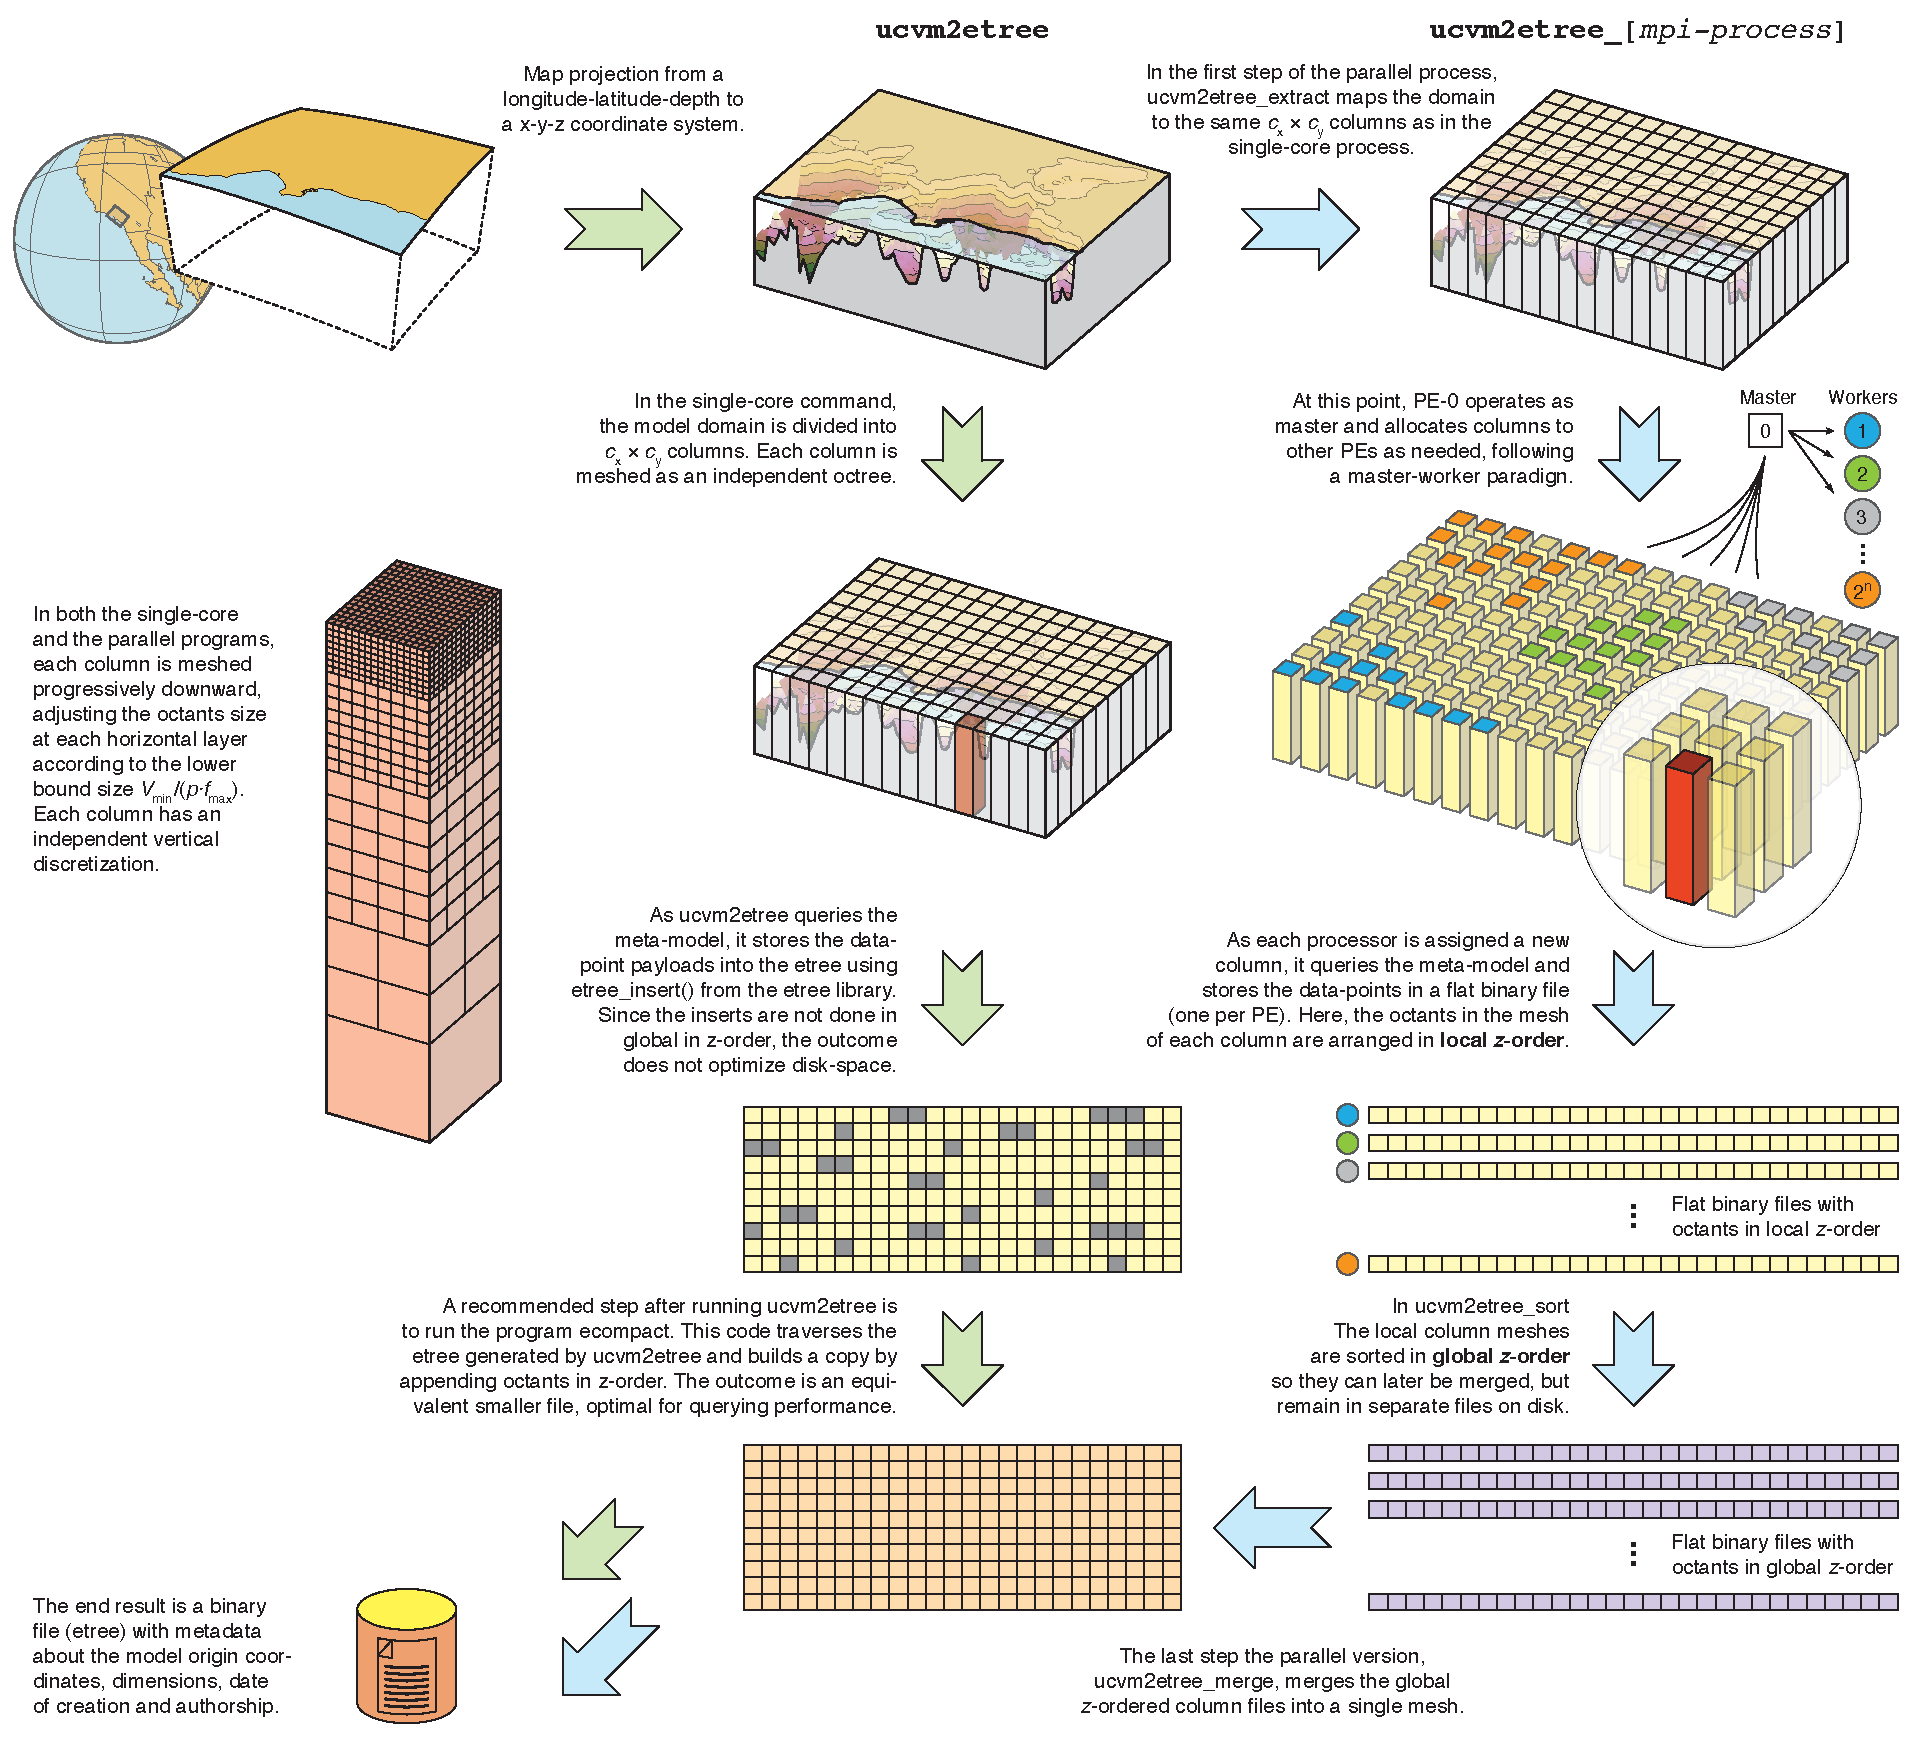
\includegraphics
		[width=\textwidth]
		{figures/pdf/ucvm-to-etree}
	\caption{Construction of an pseudo-unstructured mesh in the Etree database format using the program \texttt{ucvm2etree} and its MPI equivalent processes \texttt{ucvm2etree\_extract}, \texttt{ucvm2etree\_sort} and \texttt{ucvm2etree\_merge}. An important aspect of the meshing-to-etree process is that the discretized information payload (\vs{}, \vp{}, and $\rho$) is stored at the octants in the octree structure. The querying and assignment process mapps the information queried at the center of each octant to the whole volume enclosed by the octant.}
	\label{fig:etrees}
\end{figure*}
% ---------------------------------------------------------------------------------------------
